
\documentclass[letterpaper,hide notes,xcolor={table,svgnames},pdftex,10pt]{beamer}
\def\showexamples{t}


%\usepackage[svgnames]{xcolor}

%% Demo talk
%\documentclass[letterpaper,notes=show]{beamer}

\usecolortheme{crane}
\setbeamertemplate{navigation symbols}{}

\usetheme{MyPittsburgh}
%\usetheme{Frankfurt}

%\usepackage{tipa}

\usepackage{hyperref}
\usepackage{graphicx,xspace}
\usepackage[normalem]{ulem}
\usepackage{multicol}
\usepackage{amsmath,amssymb,amsthm,graphicx,xspace}
\newcommand\SF[1]{$\bigstar$\footnote{SF: #1}}

\usepackage[default]{sourcesanspro}
\usepackage[T1]{fontenc}
\usepackage[scaled]{beramono}
\usepackage{tikzpagenodes}

\newcounter{tmpnumSlide}
\newcounter{tmpnumNote}


% old question code
%\newcommand\question[1]{{$\bigstar$ \small \onlySlide{2}{#1}}}
% \newcommand\nquestion[1]{\ifdefined \presentationonly \textcircled{?} \fi \note{\par{\Large \textbf{?}} #1}}
% \newcommand\nanswer[1]{\note{\par{\Large \textbf{A}} #1}}


 \newcommand\mnote[1]{%
   \addtocounter{tmpnumSlide}{1}
   \ifdefined\showcues {~\tiny\fbox{\arabic{tmpnumSlide}}}\fi
   \note{\setlength{\parskip}{1ex}\addtocounter{tmpnumNote}{1}\textbf{\Large \arabic{tmpnumNote}:} {#1\par}}}

\newcommand\mmnote[1]{\note{\setlength{\parskip}{1ex}#1\par}}

%\newcommand\mnote[2][]{\ifdefined\handoutwithnotes {~\tiny\fbox{#1}}\fi
% \note{\setlength{\parskip}{1ex}\textbf{\Large #1:} #2\par}}

%\newcommand\mnote[2][]{{\tiny\fbox{#1}} \note{\setlength{\parskip}{1ex}\textbf{\Large #1:} #2\par}}

\newcommand\mquestion[2]{{~\color{red}\fbox{?}}\note{\setlength{\parskip}{1ex}\par{\Large \textbf{?}} #1} \note{\setlength{\parskip}{1ex}\par{\Large \textbf{A}} #2\par}\ifdefined \presentationonly \pause \fi}

\newcommand\blackboard[1]{%
\ifdefined   \showblackboard
  {#1}
  \else {\begin{center} \fbox{\colorbox{blue!30}{%
         \begin{minipage}{.95\linewidth}%
           \hspace{\stretch{1}} Some space intentionally left blank; done at the blackboard.%
         \end{minipage}}}\end{center}}%
         \fi%
}



%\newcommand\q{\tikz \node[thick,color=black,shape=circle]{?};}
%\newcommand\q{\ifdefined \presentationonly \textcircled{?} \fi}

\usepackage{listings}
\lstset{basicstyle=\footnotesize\ttfamily,
	breaklines=true,
	aboveskip=15pt,
  	belowskip=15pt,
	frame=lines,
	numbers=left, basicstyle=\scriptsize, numberstyle=\tiny, stepnumber=0, numbersep=2pt
}

\usepackage{siunitx}
\newcommand\sius[1]{\num[group-separator = {,}]{#1}\si{\micro\second}}
\newcommand\sims[1]{\num[group-separator = {,}]{#1}\si{\milli\second}}
\newcommand\sins[1]{\num[group-separator = {,}]{#1}\si{\nano\second}}
\sisetup{group-separator = {,}, group-digits = true}

%% -------------------- tikz --------------------
\usepackage{tikz}
\usetikzlibrary{positioning}
\usetikzlibrary{arrows,backgrounds,automata,decorations.shapes,decorations.pathmorphing,decorations.markings,decorations.text,decorations.pathreplacing}

\tikzstyle{place}=[circle,draw=blue!50,fill=blue!20,thick, inner sep=0pt,minimum size=6mm]
\tikzstyle{transition}=[rectangle,draw=black!50,fill=black!20,thick, inner sep=0pt,minimum size=4mm]

\tikzstyle{block}=[rectangle,draw=black, thick, inner sep=5pt]
\tikzstyle{bullet}=[circle,draw=black, fill=black, thin, inner sep=2pt]

\tikzstyle{pre}=[<-,shorten <=1pt,>=stealth',semithick]
\tikzstyle{post}=[->,shorten >=1pt,>=stealth',semithick]
\tikzstyle{bi}=[<->,shorten >=1pt,shorten <=1pt, >=stealth',semithick]

\tikzstyle{mut}=[-,>=stealth',semithick]

\tikzstyle{treereset}=[dashed,->, shorten >=1pt,>=stealth',thin]

\usepackage{ifmtarg}
\usepackage{xifthen}
\makeatletter
% new counter to now which frame it is within the sequence
\newcounter{multiframecounter}
% initialize buffer for previously used frame title
\gdef\lastframetitle{\textit{undefined}}
% new environment for a multi-frame
\newenvironment{multiframe}[1][]{%
\ifthenelse{\isempty{#1}}{%
% if no frame title was set via optional parameter,
% only increase sequence counter by 1
\addtocounter{multiframecounter}{1}%
}{%
% new frame title has been provided, thus
% reset sequence counter to 1 and buffer frame title for later use
\setcounter{multiframecounter}{1}%
\gdef\lastframetitle{#1}%
}%
% start conventional frame environment and
% automatically set frame title followed by sequence counter
\begin{frame}%
\frametitle{\lastframetitle~{\normalfont(\arabic{multiframecounter})}}%
}{%
\end{frame}%
}
\makeatother

\makeatletter
\newdimen\tu@tmpa%
\newdimen\ydiffl%
\newdimen\xdiffl%
\newcommand\ydiff[2]{%
    \coordinate (tmpnamea) at (#1);%
    \coordinate (tmpnameb) at (#2);%
    \pgfextracty{\tu@tmpa}{\pgfpointanchor{tmpnamea}{center}}%
    \pgfextracty{\ydiffl}{\pgfpointanchor{tmpnameb}{center}}%
    \advance\ydiffl by -\tu@tmpa%
}
\newcommand\xdiff[2]{%
    \coordinate (tmpnamea) at (#1);%
    \coordinate (tmpnameb) at (#2);%
    \pgfextractx{\tu@tmpa}{\pgfpointanchor{tmpnamea}{center}}%
    \pgfextractx{\xdiffl}{\pgfpointanchor{tmpnameb}{center}}%
    \advance\xdiffl by -\tu@tmpa%
}
\makeatother
\newcommand{\copyrightbox}[3][r]{%
\begin{tikzpicture}%
\node[inner sep=0pt,minimum size=2em](ciimage){#2};
\usefont{OT1}{phv}{n}{n}\fontsize{4}{4}\selectfont
\ydiff{ciimage.south}{ciimage.north}
\xdiff{ciimage.west}{ciimage.east}
\ifthenelse{\equal{#1}{r}}{%
\node[inner sep=0pt,right=1ex of ciimage.south east,anchor=north west,rotate=90]%
{\raggedleft\color{black!50}\parbox{\the\ydiffl}{\raggedright{}#3}};%
}{%
\ifthenelse{\equal{#1}{l}}{%
\node[inner sep=0pt,right=1ex of ciimage.south west,anchor=south west,rotate=90]%
{\raggedleft\color{black!50}\parbox{\the\ydiffl}{\raggedright{}#3}};%
}{%
\node[inner sep=0pt,below=1ex of ciimage.south west,anchor=north west]%
{\raggedleft\color{black!50}\parbox{\the\xdiffl}{\raggedright{}#3}};%
}
}
\end{tikzpicture}
}


%% --------------------

%\usepackage[excludeor]{everyhook}
%\PushPreHook{par}{\setbox0=\lastbox\llap{MUH}}\box0}

%\vspace*{\stretch{1}

%\setbox0=\lastbox \llap{\textbullet\enskip}\box0}

\setlength{\parskip}{\fill}

\newcommand\noskips{\setlength{\parskip}{1ex}}
\newcommand\doskips{\setlength{\parskip}{\fill}}

\newcommand\xx{\par\vspace*{\stretch{1}}\par}
\newcommand\xxs{\par\vspace*{2ex}\par}
\newcommand\tuple[1]{\langle #1 \rangle}
\newcommand\code[1]{{\sf \footnotesize #1}}
\newcommand\ex[1]{\uline{Example:} \ifdefined \presentationonly \pause \fi
  \ifdefined\showexamples#1\xspace\else{\uline{\hspace*{2cm}}}\fi}

\newcommand\ceil[1]{\lceil #1 \rceil}


\AtBeginSection[]
{
   \begin{frame}
       \frametitle{Outline}
       \tableofcontents[currentsection]
   \end{frame}
}



\pgfdeclarelayer{edgelayer}
\pgfdeclarelayer{nodelayer}
\pgfsetlayers{edgelayer,nodelayer,main}

\tikzstyle{none}=[inner sep=0pt]
\tikzstyle{rn}=[circle,fill=Red,draw=Black,line width=0.8 pt]
\tikzstyle{gn}=[circle,fill=Lime,draw=Black,line width=0.8 pt]
\tikzstyle{yn}=[circle,fill=Yellow,draw=Black,line width=0.8 pt]
\tikzstyle{empty}=[circle,fill=White,draw=Black]
\tikzstyle{bw} = [rectangle, draw, fill=blue!20, 
    text width=4em, text centered, rounded corners, minimum height=2em]
    
    \newcommand{\CcNote}[1]{% longname
	This work is licensed under the \textit{Creative Commons #1 3.0 License}.%
}
\newcommand{\CcImageBy}[1]{%
	\includegraphics[scale=#1]{creative_commons/cc_by_30.pdf}%
}
\newcommand{\CcImageSa}[1]{%
	\includegraphics[scale=#1]{creative_commons/cc_sa_30.pdf}%
}
\newcommand{\CcImageNc}[1]{%
	\includegraphics[scale=#1]{creative_commons/cc_nc_30.pdf}%
}
\newcommand{\CcGroupBySa}[2]{% zoom, gap
	\CcImageBy{#1}\hspace*{#2}\CcImageNc{#1}\hspace*{#2}\CcImageSa{#1}%
}
\newcommand{\CcLongnameByNcSa}{Attribution-NonCommercial-ShareAlike}

\newenvironment{changemargin}[1]{% 
  \begin{list}{}{% 
    \setlength{\topsep}{0pt}% 
    \setlength{\leftmargin}{#1}% 
    \setlength{\rightmargin}{1em}
    \setlength{\listparindent}{\parindent}% 
    \setlength{\itemindent}{\parindent}% 
    \setlength{\parsep}{\parskip}% 
  }% 
  \item[]}{\end{list}} 




\title{Lecture 12 --- OpenMP }

\author{Patrick Lam \\ \small \texttt{patrick.lam@uwaterloo.ca}}
\institute{Department of Electrical and Computer Engineering \\
  University of Waterloo}
\date{\today}


\begin{document}

\begin{frame}
  \titlepage

 \end{frame}

{ % all template changes are local to this group.
    \setbeamertemplate{navigation symbols}{}
    \begin{frame}[plain]
        \begin{tikzpicture}[remember picture,overlay]
            \node[at=(current page.center)] (pic) {
                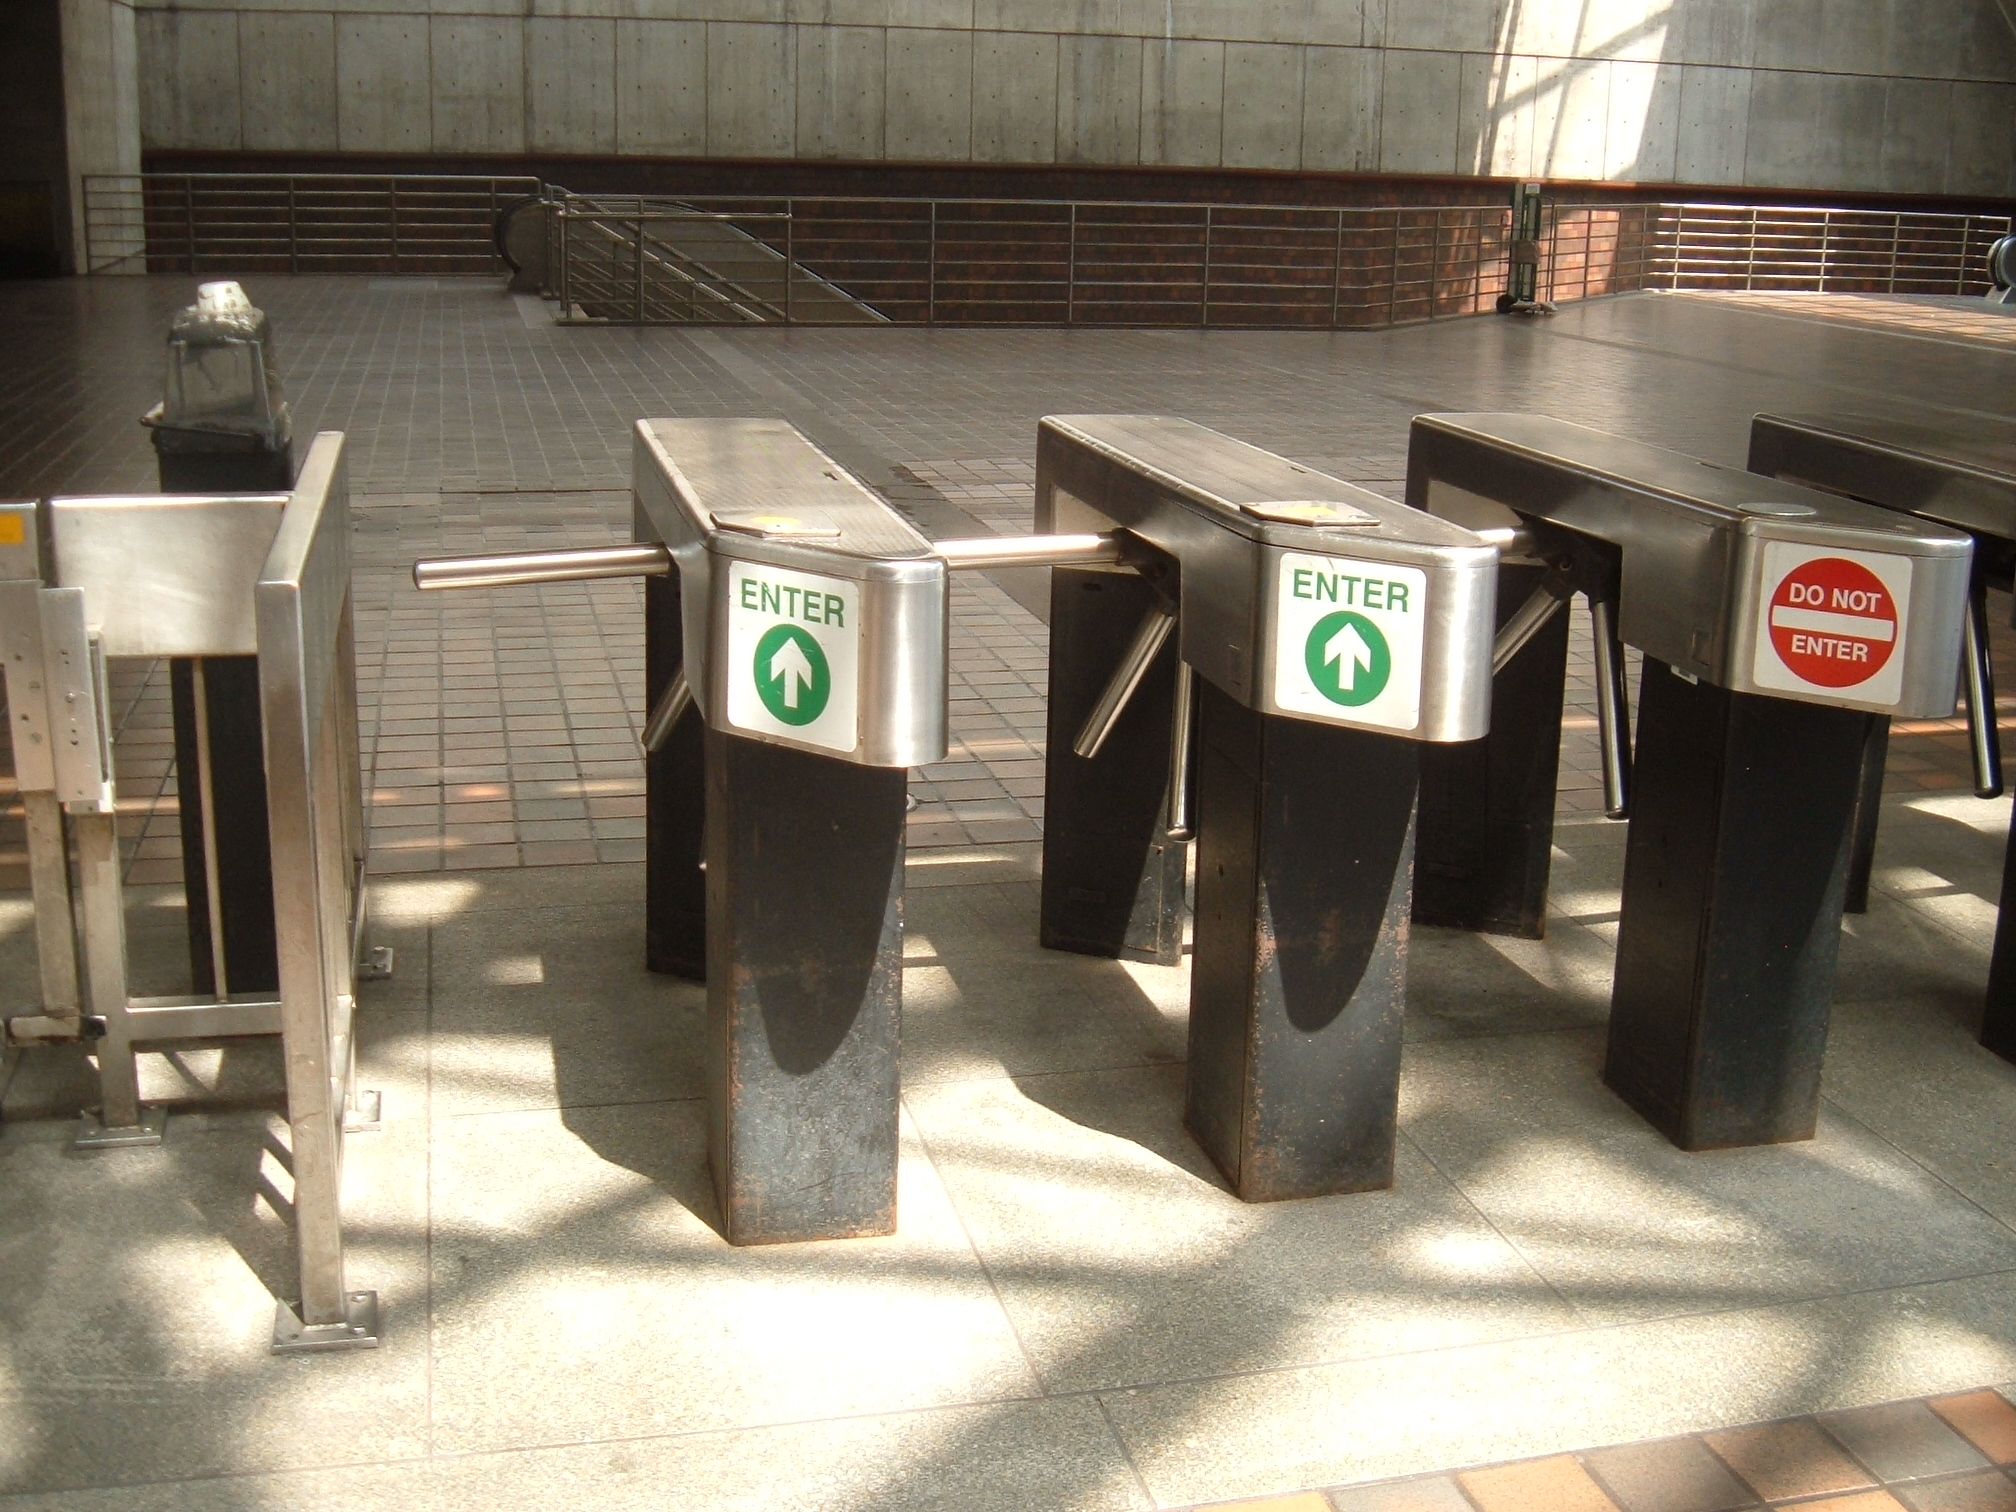
\includegraphics[width=\paperwidth]{images/L12-turnstile-alewife.jpg}
            };
%            \draw node (current page.south) {Hello};
            \node[anchor=south] at (current page text area.south) { photo: Arnold Reinhold via Wikimedia Commons };
        \end{tikzpicture}
     \end{frame}
}

%%%%%%%%%%%%%%%%%%%%%%%%%%%%%%%%%%%%%%%%%%%%%%%%%%%%%%%%%%%%%%%%%%%%%%%%%%%%%%%%
\begin{frame}[containsverbatim]
  \frametitle{Context for OpenMP}

\vspace*{-3em}
\Large
\begin{changemargin}{1.5cm}
    So far: Pthreads and \\
          \hspace*{4em}automatic parallelization.\\[1em]
    Next: ``Manual'' parallelization \\
          \hspace*{4em}using OpenMP.
\end{changemargin}

\end{frame}
%%%%%%%%%%%%%%%%%%%%%%%%%%%%%%%%%%%%%%%%%%%%%%%%%%%%%%%%%%%%%%%%%%%%%%%%%%%%%%%%

%%%%%%%%%%%%%%%%%%%%%%%%%%%%%%%%%%%%%%%%%%%%%%%%%%%%%%%%%%%%%%%%%%%%%%%%%%%%%%%%
\begin{frame}[containsverbatim]
  \frametitle{What is OpenMP?}

\vspace*{-3em}  
\Large
\begin{changemargin}{1.5cm}
    OpenMP = Open Multiprocessing.\\[2em]
    You specify parallelization; \\
    \hspace*{4em} compiler implements.\\[1em]
    ``I want 10 turnstiles.''
\end{changemargin}

\end{frame}
%%%%%%%%%%%%%%%%%%%%%%%%%%%%%%%%%%%%%%%%%%%%%%%%%%%%%%%%%%%%%%%%%%%%%%%%%%%%%%%%

%%%%%%%%%%%%%%%%%%%%%%%%%%%%%%%%%%%%%%%%%%%%%%%%%%%%%%%%%%%%%%%%%%%%%%%%%%%%%%%%
\begin{frame}[containsverbatim]
  \frametitle{OpenMP Compiler Support}
\vspace*{-3em}
\Large
\begin{changemargin}{1.5cm}
    All major compilers have OpenMP \\
    \qquad (GCC, clang, Solaris,
      Intel, Microsoft).\\[1em]

  Use OpenMP\footnote{More information:
    \url{https://computing.llnl.gov/tutorials/openMP/}} by specifying\\
  \hspace*{4em} directives in source code. \\[1em]
  C/C++: pragmas of the
  form \verb+#pragma omp ...+
\end{changemargin}
\end{frame}
%%%%%%%%%%%%%%%%%%%%%%%%%%%%%%%%%%%%%%%%%%%%%%%%%%%%%%%%%%%%%%%%%%%%%%%%%%%%%%%%

%%%%%%%%%%%%%%%%%%%%%%%%%%%%%%%%%%%%%%%%%%%%%%%%%%%%%%%%%%%%%%%%%%%%%%%%%%%%%%%%
\begin{frame}
  \frametitle{Benefits of OpenMP}

\large
  
\begin{changemargin}{1.5cm}
  \begin{itemize}
    \item uses compiler directives---
      \begin{itemize}
        \item easily compile same codebase for serial or parallel.
      \end{itemize}
    \item separates parallelization implementation\\
      from algorithm implementation.
   \end{itemize}~\\[-2em]

    Directives apply to limited parts of the code, \\
    enabling incremental parallelization of the program.\\
    (Start with the hotspots.)
\end{changemargin}
\end{frame}
%%%%%%%%%%%%%%%%%%%%%%%%%%%%%%%%%%%%%%%%%%%%%%%%%%%%%%%%%%%%%%%%%%%%%%%%%%%%%%%%

%%%%%%%%%%%%%%%%%%%%%%%%%%%%%%%%%%%%%%%%%%%%%%%%%%%%%%%%%%%%%%%%%%%%%%%%%%%%%%%%
\begin{frame}[fragile]
  \frametitle{Simple OpenMP Example}

  
  \begin{lstlisting}[language=C,morekeywords={foreach,pragma,omp,parallel,single,nowait,task,untied,barrier,taskyield}]
void calc (double *array1, double *array2, int length) {
    #pragma omp parallel for
    for (int i = 0; i < length; i++) {
        array1[i] += array2[i];
    }
}
  \end{lstlisting}

\Large
\begin{changemargin}{.5cm}
  Without OpenMP: \\ \quad Could compiler parallelize this automatically?
\end{changemargin}

\end{frame}
%%%%%%%%%%%%%%%%%%%%%%%%%%%%%%%%%%%%%%%%%%%%%%%%%%%%%%%%%%%%%%%%%%%%%%%%%%%%%%%%

%%%%%%%%%%%%%%%%%%%%%%%%%%%%%%%%%%%%%%%%%%%%%%%%%%%%%%%%%%%%%%%%%%%%%%%%%%%%%%%%
\begin{frame}[containsverbatim]
  \frametitle{How The Example Works}

\large
  
    \verb+#pragma+ will force the compiler to parallelize the loop.

  \begin{itemize}
    \item It does not look at loop contents, only loop bounds.
    \item \alert{It is your responsibility to make sure the code is safe.}
  \end{itemize}
  OpenMP will always start parallel threads if you tell it to,\\
  dividing iterations contiguously among the threads.\\[1em]

  You don't need to declare {\tt restrict}, but it's a good idea.\\
  Need {\tt restrict} for auto-parallelization (non-OpenMP).
  

\end{frame}
%%%%%%%%%%%%%%%%%%%%%%%%%%%%%%%%%%%%%%%%%%%%%%%%%%%%%%%%%%%%%%%%%%%%%%%%%%%%%%%%

%%%%%%%%%%%%%%%%%%%%%%%%%%%%%%%%%%%%%%%%%%%%%%%%%%%%%%%%%%%%%%%%%%%%%%%%%%%%%%%%
\begin{frame}[containsverbatim]
  \frametitle{Basic {\tt pragma} syntax}

\begin{changemargin}{1cm}
\large
  Let's look at the parts of this \verb+#pragma+.\\[1em]

  \begin{itemize}
    \item \verb+#pragma omp+ indicates an OpenMP directive;
    \vfill
    \item {\tt parallel} indicates the start of a parallel region.
    \vfill
    \item {\tt for} tells OpenMP: run the next {\tt for} loop in parallel.
  \end{itemize}
  ~\\[-1em]

  When you run the parallelized program, \\ the runtime library starts
  a number of threads \& \\  assigns a subrange of the range to 
  each of the threads.
\end{changemargin}

\end{frame}
%%%%%%%%%%%%%%%%%%%%%%%%%%%%%%%%%%%%%%%%%%%%%%%%%%%%%%%%%%%%%%%%%%%%%%%%%%%%%%%%

%%%%%%%%%%%%%%%%%%%%%%%%%%%%%%%%%%%%%%%%%%%%%%%%%%%%%%%%%%%%%%%%%%%%%%%%%%%%%%%%
\begin{frame}[fragile]
  \frametitle{What OpenMP can Parallelize}

  
\begin{verbatim}
    for (int i = 0; i < length; i++) { ... }
\end{verbatim}~\\[1em]

    Can only parallelize loops which satisfy these conditions:
\begin{itemize}
\item must be of the form:\\{\tt ~~for (init expr; test expr; increment expr)};
\item loop variable must be integer (signed or unsigned), pointer, or a C++
random access iterator;
\item loop variable must be initialized to one end of the range;
\item loop increment amount must be loop-invariant (constant with respect to the loop body); and
\item test expression must be one of {\tt >}, {\tt >=}, {\tt <}, or {\tt <=}, and the comparison value (bound) must be loop-invariant.
\end{itemize}

{\bf Note:} these restrictions therefore also apply to automatically parallelized
loops.
  

\end{frame}
%%%%%%%%%%%%%%%%%%%%%%%%%%%%%%%%%%%%%%%%%%%%%%%%%%%%%%%%%%%%%%%%%%%%%%%%%%%%%%%%

%%%%%%%%%%%%%%%%%%%%%%%%%%%%%%%%%%%%%%%%%%%%%%%%%%%%%%%%%%%%%%%%%%%%%%%%%%%%%%%%
\begin{frame}[containsverbatim]
  \frametitle{What OpenMP Does}

  
  \begin{itemize}
    \item Compiler generates code to spawn a \structure{team}
of threads; automatically splits off worker-thread code into a
separate procedure.
    \item Generated code uses {\tt fork-join} parallelism; when the
master thread hits a parallel region, it gives work to the worker
threads, which execute and report back.
    \item Afterwards, the master thread
continues running, while the worker threads wait for more work .
  \end{itemize}

~\\
As we saw, you can specify the number of threads by setting the
\verb+OMP_NUM_THREADS+ environment variable. (You can also adjust by calling 
\verb+omp_set_num_threads()+).

\begin{itemize}
  \item Solaris compiler tells you what it did if you use the flags \verb+-xopenmp -xloopinfo+, or \verb+er_src+.
\end{itemize}

  


\end{frame}
%%%%%%%%%%%%%%%%%%%%%%%%%%%%%%%%%%%%%%%%%%%%%%%%%%%%%%%%%%%%%%%%%%%%%%%%%%%%%%%%

%%%%%%%%%%%%%%%%%%%%%%%%%%%%%%%%%%%%%%%%%%%%%%%%%%%%%%%%%%%%%%%%%%%%%%%%%%%%%%%%
\begin{frame}[fragile]
  \frametitle{Variable Scoping}

  

  Concept: thread-local variables (\structure{private})
      vs shared~variables.
  \begin{itemize}
    \item Writes to private variables:\\
\qquad visible only to writing thread.
    \item Writes to shared variables:\\ 
\qquad visible to all threads.
  \end{itemize}

  

\end{frame}
%%%%%%%%%%%%%%%%%%%%%%%%%%%%%%%%%%%%%%%%%%%%%%%%%%%%%%%%%%%%%%%%%%%%%%%%%%%%%%%%

%%%%%%%%%%%%%%%%%%%%%%%%%%%%%%%%%%%%%%%%%%%%%%%%%%%%%%%%%%%%%%%%%%%%%%%%%%%%%%%%
\begin{frame}[fragile]
  \frametitle{Variable Scoping for Example}

  

\begin{verbatim}
    for (int i = 0; i < length; i++) { ... }
\end{verbatim}

\large
  \begin{itemize}
    \item {\tt length} could be either shared or private.
    \begin{itemize}
      \item if it was private, then you would have to copy
in the appropriate initial value.
    \end{itemize}
    \item {\tt array} variables must be shared.
  \end{itemize}
  

\end{frame}

%%%%%%%%%%%%%%%%%%%%%%%%%%%%%%%%%%%%%%%%%%%%%%%%%%%%%%%%%%%%%%%%%%%%%%%%%%%%%%%%

%%%%%%%%%%%%%%%%%%%%%%%%%%%%%%%%%%%%%%%%%%%%%%%%%%%%%%%%%%%%%%%%%%%%%%%%%%%%%%%%
\begin{frame}[fragile]
  \frametitle{Default Variable Scoping}
  
Let's look at the defaults that OpenMP uses to parallelize the {\tt parallel-for} code:
\begin{lstlisting}
% er_src parallel-for.o
     1.   <Function: calc>
    
    Source OpenMP region below has tag R1
    Private variables in R1: i
    Shared variables in R1: array2, length, array1
     2.     #pragma omp parallel for
\end{lstlisting}
  

\end{frame}

%%%%%%%%%%%%%%%%%%%%%%%%%%%%%%%%%%%%%%%%%%%%%%%%%%%%%%%%%%%%%%%%%%%%%%%%%%%%%%%%

%%%%%%%%%%%%%%%%%%%%%%%%%%%%%%%%%%%%%%%%%%%%%%%%%%%%%%%%%%%%%%%%%%%%%%%%%%%%%%%%
\begin{frame}[fragile]
  \frametitle{Parallelization information (via OpenMP)}
\begin{lstlisting}
    Source loop below has tag L1
    L1 autoparallelized
    L1 parallelized by explicit user directive
    L1 parallel loop-body code placed in function _$d1A2.calc 
                     along with 0 inner loops
    L1 multi-versioned for loop-improvement:
                     dynamic-alias-disambiguation. 
        Specialized version is L2
     3.     for (int i = 0; i < length; i++) {
     4.       array1[i] += array2[i];
     5.     }
     6.   }
\end{lstlisting}

\end{frame}

%%%%%%%%%%%%%%%%%%%%%%%%%%%%%%%%%%%%%%%%%%%%%%%%%%%%%%%%%%%%%%%%%%%%%%%%%%%%%%%%

%%%%%%%%%%%%%%%%%%%%%%%%%%%%%%%%%%%%%%%%%%%%%%%%%%%%%%%%%%%%%%%%%%%%%%%%%%%%%%%%
\begin{frame}[fragile]
  \frametitle{Default Variable Scoping Rules: A Summary}


\begin{itemize}
  \item Loop variables are private.
  \item Variables defined in parallel code are private.
  \item Variables defined outside the parallel region are shared.
\end{itemize}
~\\

You can disable the default rules \\
by specifying {\tt default(none)} on the {\tt parallel} pragma, \\
or you can give explicit scoping:

\begin{lstlisting}
#pragma omp parallel for private(i) 
                         shared(length, array1, array2)
\end{lstlisting}
  


\end{frame}
%%%%%%%%%%%%%%%%%%%%%%%%%%%%%%%%%%%%%%%%%%%%%%%%%%%%%%%%%%%%%%%%%%%%%%%%%%%%%%%%

%%%%%%%%%%%%%%%%%%%%%%%%%%%%%%%%%%%%%%%%%%%%%%%%%%%%%%%%%%%%%%%%%%%%%%%%%%%%%%%%
\begin{frame}[fragile]
  \frametitle{Reductions}
  
Recall that we introduced the concept of a reduction, e.g.
\begin{lstlisting}[language=C,morekeywords={foreach,pragma,omp,parallel,single,nowait,task,untied,barrier,taskyield}]
for (int i = 0; i < length; i++)
    total += array[i];
\end{lstlisting}

What is the appropriate scope for {\tt total}? \\
\pause
Well, it should be
\structure{shared}.

\begin{itemize}
 \item We want each thread to be able to write to it. \pause
 \item But, is there a race condition? (of course)
\end{itemize}

Aha! OpenMP can deal with reductions as a special case:


\begin{lstlisting}
#pragma omp parallel for reduction (+:total)
\end{lstlisting}

specifies that the {\tt total} variable is the accumulator for a
reduction over the {\tt +} operator.
  

\end{frame}
%%%%%%%%%%%%%%%%%%%%%%%%%%%%%%%%%%%%%%%%%%%%%%%%%%%%%%%%%%%%%%%%%%%%%%%%%%%%%%%%


%%%%%%%%%%%%%%%%%%%%%%%%%%%%%%%%%%%%%%%%%%%%%%%%%%%%%%%%%%%%%%%%%%%%%%%%%%%%%%%%
\begin{frame}[fragile]
  \frametitle{Accessing Private Data outside a Parallel Region}

  
Sometimes you want \structure{private} variables, but want them initialized
before the loop.\\[1em]

Consider this (silly) code:

\begin{lstlisting}
int data=1;
#pragma omp parallel for private(data)
for (int i = 0; i < 100; i++)
    printf ("data=%d\n", data);
\end{lstlisting}


\begin{itemize}
  \item {\tt data} is private, so OpenMP will not copy in initial 1.
  \item To make OpenMP copy the data before the threads start, use
    {\tt firstprivate(data)}.
  \item To publish a variable after the (sequentially) last iteration of the loop, use
    {\tt lastprivate(data)}.
\end{itemize}
  

\end{frame}
%%%%%%%%%%%%%%%%%%%%%%%%%%%%%%%%%%%%%%%%%%%%%%%%%%%%%%%%%%%%%%%%%%%%%%%%%%%%%%%%

%%%%%%%%%%%%%%%%%%%%%%%%%%%%%%%%%%%%%%%%%%%%%%%%%%%%%%%%%%%%%%%%%%%%%%%%%%%%%%%%
\begin{frame}
  \frametitle{Thread-Private Data}

  

    You might have a global variable, for which each thread should have a persistent local copy---lives across parallel regions.\\[1em]
  \begin{itemize}
    \item Use the {\tt threadprivate} directive.
    \item Add {\tt copyin} if you want something like
      {\tt firstprivate}.
    \item There is no {\tt lastprivate} since the data is accessible after the
      loop.
  \end{itemize}
  

\end{frame}
%%%%%%%%%%%%%%%%%%%%%%%%%%%%%%%%%%%%%%%%%%%%%%%%%%%%%%%%%%%%%%%%%%%%%%%%%%%%%%%%

%%%%%%%%%%%%%%%%%%%%%%%%%%%%%%%%%%%%%%%%%%%%%%%%%%%%%%%%%%%%%%%%%%%%%%%%%%%%%%%%
\begin{frame}[fragile]
  \frametitle{Thread-Private Data Example (1)}

  
  \begin{lstlisting}[language=C,morekeywords={foreach,pragma,omp,parallel,single,nowait,task,untied,barrier,taskyield}]
#include <omp.h>
#include <stdio.h>

int tid, a, b;

#pragma omp threadprivate(a)

int main(int argc, char *argv[])
{
    printf("Parallel #1 Start\n");
    #pragma omp parallel private(b, tid)
    {
        tid = omp_get_thread_num();
        a = tid;
        b = tid;
        printf("T%d: a=%d, b=%d\n", tid, a, b);
    }

    printf("Sequential code\n");
  \end{lstlisting}
  


\end{frame}
%%%%%%%%%%%%%%%%%%%%%%%%%%%%%%%%%%%%%%%%%%%%%%%%%%%%%%%%%%%%%%%%%%%%%%%%%%%%%%%%

%%%%%%%%%%%%%%%%%%%%%%%%%%%%%%%%%%%%%%%%%%%%%%%%%%%%%%%%%%%%%%%%%%%%%%%%%%%%%%%%
\begin{frame}[fragile]
  \frametitle{Thread-Private Data Example (2)}

  
  \begin{lstlisting}[language=C,morekeywords={foreach,pragma,omp,parallel,single,nowait,task,untied,barrier,taskyield}]
    printf("Parallel #2 Start\n");
    #pragma omp parallel private(tid)
    {
        tid = omp_get_thread_num();
        printf("T%d: a=%d, b=%d\n", tid, a, b);
    }

    return 0;
}    
  \end{lstlisting}
  
  
  \begin{center}
    \begin{columns}[c]
      \column{1.5in}
        \begin{lstlisting}
% ./a.out
Parallel #1 Start
T6: a=6, b=6
T1: a=1, b=1
T0: a=0, b=0
T4: a=4, b=4
T2: a=2, b=2
T3: a=3, b=3
T5: a=5, b=5
T7: a=7, b=7
        \end{lstlisting}
      \column{1.5in}
        \begin{lstlisting}
Sequential code
Parallel #2 Start
T0: a=0, b=0
T6: a=6, b=0
T1: a=1, b=0
T2: a=2, b=0
T5: a=5, b=0
T7: a=7, b=0
T3: a=3, b=0
T4: a=4, b=0
        \end{lstlisting}
    \end{columns}
  \end{center}
\end{frame}
%%%%%%%%%%%%%%%%%%%%%%%%%%%%%%%%%%%%%%%%%%%%%%%%%%%%%%%%%%%%%%%%%%%%%%%%%%%%%%%%

%%%%%%%%%%%%%%%%%%%%%%%%%%%%%%%%%%%%%%%%%%%%%%%%%%%%%%%%%%%%%%%%%%%%%%%%%%%%%%%%
\begin{frame}[fragile]
  \frametitle{Atomic}

  \Large
  \begin{changemargin}{1.5cm}
  \begin{center}
    {\tt \#pragma omp }{\bf atomic} [{\bf read $\mid$ write $\mid$ update $\mid$ capture}]\\
    {\it expression-stmt}
  \end{center}~\\

    Ensures a specific storage location is updated atomically.\\[1em]
    More efficient than using critical sections \\
      \hspace*{2em} (or else why would they
      include it?)\\[2em]

  \end{changemargin}

\end{frame}
%%%%%%%%%%%%%%%%%%%%%%%%%%%%%%%%%%%%%%%%%%%%%%%%%%%%%%%%%%%%%%%%%%%%%%%%%%%%%%%%

%%%%%%%%%%%%%%%%%%%%%%%%%%%%%%%%%%%%%%%%%%%%%%%%%%%%%%%%%%%%%%%%%%%%%%%%%%%%%%%%
\begin{frame}[fragile]
  \frametitle{Atomic Expressions}

  \begin{changemargin}{1cm}

  {\bf read expression:} {\tt v = x;}\\[1em]

  {\bf write expression:} {\tt x = expr;}\\[1em]

  {\bf update expression:} {\tt x++;} {\tt x{-}-;} {\tt ++x;} {\tt -{-}x;}\\
  \hspace{9em}{\tt x binop= expr;} {\tt x = x binop expr;}\\[1em]

    {\tt expr} must not access the same location as {\tt v} or {\tt x}.\\
    {\tt v} and {\tt x} must not access the same location; must be
      primitives.\\
    All operations to {\tt x} are atomic.\\[2em]

  {\bf capture expression:} {\tt v = x++;} {\tt v = x{-}-;} {\tt v = ++x;}
  {\tt v = -{-}x;}\\ \hspace{9.2em}{\tt v = x binop= expr;}

  Performs the indicated update. Also stores the original or
  final value computed.
  \end{changemargin}

\end{frame}
%%%%%%%%%%%%%%%%%%%%%%%%%%%%%%%%%%%%%%%%%%%%%%%%%%%%%%%%%%%%%%%%%%%%%%%%%%%%%%%%

%%%%%%%%%%%%%%%%%%%%%%%%%%%%%%%%%%%%%%%%%%%%%%%%%%%%%%%%%%%%%%%%%%%%%%%%%%%%%%%%
\begin{frame}[fragile]
  \frametitle{Collapsing Loops}


  \begin{itemize}
    \item Normally, it's best to parallelize the outermost loop.
  \end{itemize}

  

  ~\\
  Consider this code:

  \begin{lstlisting}[language=C,morekeywords={foreach,pragma,omp,parallel,single,nowait,task,untied,barrier,taskyield}]
#include <math.h>
int main() {
    double array[2][10000];
    #pragma omp parallel for collapse(2)
    for (int i = 0; i < 2; i++)
      for (int j = 0; j < 10000; j++)
        array[i][j] = sin(i+j);
    return 0;
}
  \end{lstlisting}


  \begin{itemize}
  \item Would parallelizing this outer loop benefit us?\\
    What about the inner loop?
  \end{itemize}

  OpenMP supports \emph{collapsing} loops:

  \begin{itemize}
    \item Creates a single loop for all the iterations of the two loops.
    \item Outer loop only enables the use of 2 threads.
    \item Collapsed loop lets us use up to 20,000 threads.
  \end{itemize}
  

\end{frame}
%%%%%%%%%%%%%%%%%%%%%%%%%%%%%%%%%%%%%%%%%%%%%%%%%%%%%%%%%%%%%%%%%%%%%%%%%%%%%%%%


%%%%%%%%%%%%%%%%%%%%%%%%%%%%%%%%%%%%%%%%%%%%%%%%%%%%%%%%%%%%%%%%%%%%%%%%%%%%%%%%
\begin{frame}[fragile]
  \frametitle{Better Performance Through Scheduling: An Example}

  

  Default mode: \emph{Static scheduling}.
  \begin{itemize}
    \item Assumes each iteration takes the same running time.
  \end{itemize}

  Does that assumption hold for this code?

  \begin{lstlisting}[language=C,morekeywords={foreach,pragma,omp,parallel,single,nowait,task,untied,barrier,taskyield}]
double calc(int count) {
    double d = 1.0;
    for (int i = 0; i < count*count; i++) d += d;
    return d;
}

int main() {
    double data[200][100];
    int i, j;
    #pragma omp parallel for private(i, j) shared(data)
    for (int i = 0; i < 200; i++) {
        for (int j = 0; j < 200; j++) {
            data[i][j] = calc(i+j);
        }
    }
    return 0;
}
  \end{lstlisting}
  

\end{frame}
%%%%%%%%%%%%%%%%%%%%%%%%%%%%%%%%%%%%%%%%%%%%%%%%%%%%%%%%%%%%%%%%%%%%%%%%%%%%%%%%

%%%%%%%%%%%%%%%%%%%%%%%%%%%%%%%%%%%%%%%%%%%%%%%%%%%%%%%%%%%%%%%%%%%%%%%%%%%%%%%%
\begin{frame}[fragile]
  \frametitle{Better Performance Through Scheduling}

\large

  
  \begin{itemize}
    \item In example, earlier iterations are faster than later iterations.\\
          Result: sublinear scaling---wait for all iterations to finish.\\[1em]
    \item Turn on \emph{dynamic schedule} mode\\ by adding
      {\tt schedule(dynamic)} to the pragma:
      \begin{itemize}
        \item Breaks the work into chunks;
        \item Distributes the work to each thread in chunks;
        \item Higher overhead;
        \item Default chunk size of 1\\ (can modify, e.g. {\tt schedule(dynamic, n/50)}).
      \end{itemize}
  \end{itemize}
  


\end{frame}
%%%%%%%%%%%%%%%%%%%%%%%%%%%%%%%%%%%%%%%%%%%%%%%%%%%%%%%%%%%%%%%%%%%%%%%%%%%%%%%%

%%%%%%%%%%%%%%%%%%%%%%%%%%%%%%%%%%%%%%%%%%%%%%%%%%%%%%%%%%%%%%%%%%%%%%%%%%%%%%%%
\begin{frame}[fragile]
  \frametitle{More Scheduling}

  
  
  Other schedule modes exist, e.g. {\tt guided}, {\tt auto} and {\tt runtime}.
      
  \begin{itemize}
    \item {\tt guided} changes the chunk size based on work
          remaining.
          
      \begin{itemize}
        \item Default minimum chunk size = 1 (can modify)
      \end{itemize}
    \item {\tt auto} lets OpenMP decide what's best.
    \item {\tt runtime} doesn't pick a mode until runtime.
      \begin{itemize}
        \item Tune with \verb+OMP_SCHEDULE+ environment variable
      \end{itemize}
  \end{itemize}
  

\end{frame}
%%%%%%%%%%%%%%%%%%%%%%%%%%%%%%%%%%%%%%%%%%%%%%%%%%%%%%%%%%%%%%%%%%%%%%%%%%%%%%%%


%%%%%%%%%%%%%%%%%%%%%%%%%%%%%%%%%%%%%%%%%%%%%%%%%%%%%%%%%%%%%%%%%%%%%%%%%%%%%%%%
\begin{frame}[fragile]
  \frametitle{Why more than for?}

\large
  
  So far, we can parallelize (some) {\tt for} loops with OpenMP.\\[1em]

  Less powerful than Pthreads. (Also harder to get wrong.)\\[1em]

  Reflects OpenMP's scientific-computation heritage.\\[1em]

  Today, we need more general parallelism, not just matrices.
  


\end{frame}
%%%%%%%%%%%%%%%%%%%%%%%%%%%%%%%%%%%%%%%%%%%%%%%%%%%%%%%%%%%%%%%%%%%%%%%%%%%%%%%%

%%%%%%%%%%%%%%%%%%%%%%%%%%%%%%%%%%%%%%%%%%%%%%%%%%%%%%%%%%%%%%%%%%%%%%%%%%%%%%%%
\begin{frame}[fragile]
  \frametitle{Parallel Sections Example: Linked Lists (1)}

\large
  
  Purely-static mechanism for specifying independent work units which should run in
  parallel.\\[1em]

  Linked list example:

{\small
\begin{lstlisting}[language=C,morekeywords={foreach,pragma,omp,parallel,single,nowait,task,untied,barrier,taskyield}]
  #include <stdlib.h>

  typedef struct s { struct s* next; } S;

  void setuplist (S* current) {
    for (int i = 0; i < 10000; i++) {
      current->next = (S*) malloc (sizeof(S));
      current = current->next;
    }
    current->next = NULL;
  }
  \end{lstlisting}
}

  


\end{frame}
%%%%%%%%%%%%%%%%%%%%%%%%%%%%%%%%%%%%%%%%%%%%%%%%%%%%%%%%%%%%%%%%%%%%%%%%%%%%%%%%

%%%%%%%%%%%%%%%%%%%%%%%%%%%%%%%%%%%%%%%%%%%%%%%%%%%%%%%%%%%%%%%%%%%%%%%%%%%%%%%%
\begin{frame}[fragile]
  \frametitle{Parallel Sections Example: Linked Lists (2)}
  

  (Exactly) 2 linked lists:
{\small
  \begin{lstlisting}
  int main() {
    S var1, var2;
    #pragma omp parallel sections
    {
      #pragma omp section
      { setuplist (&var1); }
      #pragma omp section
      { setuplist (&var2); }
    }
    return 0;
  }
\end{lstlisting}}

  Parallelism structure explicitly visible.\\[1em]
  Finite number of threads.\\[1em]
  (What's another barrier to parallelism here?)

  


\end{frame}
%%%%%%%%%%%%%%%%%%%%%%%%%%%%%%%%%%%%%%%%%%%%%%%%%%%%%%%%%%%%%%%%%%%%%%%%%%%%%%%%


%%%%%%%%%%%%%%%%%%%%%%%%%%%%%%%%%%%%%%%%%%%%%%%%%%%%%%%%%%%%%%%%%%%%%%%%%%%%%%%%
\begin{frame}[fragile]
  \frametitle{Nested Parallelism}
  

  Sometimes you don't want to collapse loops.\\[1em]

  Example: (better example in PDF notes!)\\[1em]

{\small
  \begin{lstlisting}[language=C,morekeywords={foreach,pragma,omp,parallel,single,nowait,task,untied,barrier,taskyield}]
    #pragma omp parallel sections
    {
      #pragma omp section
      { 
          #pragma omp parallel for
          for (int i = 0; i < 1000; i++) { ... } 
      }
      #pragma omp section
      {
          #pragma omp parallel for
          for (int i = 0; i < 1000; i++) { ... } 
      }
    }
\end{lstlisting}}

  To enable nested parallelism, call \verb+omp_set_nested(1)+ or
  set \verb+OMP_NESTED+. (Runtime might refuse.)\\[1em]

  
  


\end{frame}
%%%%%%%%%%%%%%%%%%%%%%%%%%%%%%%%%%%%%%%%%%%%%%%%%%%%%%%%%%%%%%%%%%%%%%%%%%%%%%%%

%%%%%%%%%%%%%%%%%%%%%%%%%%%%%%%%%%%%%%%%%%%%%%%%%%%%%%%%%%%%%%%%%%%%%%%%%%%%%%%%
\begin{frame}[fragile]
  \frametitle{OpenMP Tasks}
  

  Main new feature in OpenMP 3.0.\\[1em]

  \verb+#pragma omp task+:\\ \qquad code splits off and scheduled to run later.\\[1em]

  More flexible than parallel sections: 
  \begin{itemize}
   \item can run as many threads as needed;
   \item tasks do not need to join (like detached threads).
  \end{itemize}
  OpenMP does the task-to-thread mapping---lower overhead.

  


\end{frame}
%%%%%%%%%%%%%%%%%%%%%%%%%%%%%%%%%%%%%%%%%%%%%%%%%%%%%%%%%%%%%%%%%%%%%%%%%%%%%%%%

%%%%%%%%%%%%%%%%%%%%%%%%%%%%%%%%%%%%%%%%%%%%%%%%%%%%%%%%%%%%%%%%%%%%%%%%%%%%%%%%
\begin{frame}
  \frametitle{Examples of tasks}
  

\Large
   Two examples:
   \begin{itemize}
     \item web server\\ \quad unstructured requests
     \item user interface\\ \quad allows users to start concurrent tasks
   \end{itemize}

  


\end{frame}
%%%%%%%%%%%%%%%%%%%%%%%%%%%%%%%%%%%%%%%%%%%%%%%%%%%%%%%%%%%%%%%%%%%%%%%%%%%%%%%%

%%%%%%%%%%%%%%%%%%%%%%%%%%%%%%%%%%%%%%%%%%%%%%%%%%%%%%%%%%%%%%%%%%%%%%%%%%%%%%%%
\begin{frame}[fragile]
  \frametitle{Boa webserver main loop example}
  

{\small
\begin{lstlisting}[language=C,morekeywords={foreach,pragma,omp,parallel,single,nowait,task,untied,barrier,taskyield}]
#pragma omp parallel
  /* a single thread manages the connections */
  #pragma omp single nowait
  while (!end) {
    process any signals
    foreach request from the blocked queue {
      if (request dependencies are met) {
        extract from the blocked queue
        /* create a task for the request */
        #pragma omp task untied
          serve_request(request);
      }
    }
    if (new connection) {
      accept_connection();
      /* create a task for the request */
      #pragma omp task untied
        serve_request(new connection);
    }
    select();
  }
\end{lstlisting}
}

  


\end{frame}
%%%%%%%%%%%%%%%%%%%%%%%%%%%%%%%%%%%%%%%%%%%%%%%%%%%%%%%%%%%%%%%%%%%%%%%%%%%%%%%%

%%%%%%%%%%%%%%%%%%%%%%%%%%%%%%%%%%%%%%%%%%%%%%%%%%%%%%%%%%%%%%%%%%%%%%%%%%%%%%%%
\begin{frame}[fragile]
  \frametitle{Other OpenMP qualifiers}

  
    {\tt untied}: lifts restrictions on task-to-thread mapping.\\[1em]

    {\tt single}: only one thread runs the next statement (not $N$ copies).\\[1em]

    {\tt flush} directive: write all values in registers or cache to memory.\\[1em]

    {\tt barrier}: wait for all threads to complete. (OpenMP also has implicit
barriers at ends of parallel sections.)\\[1em]

    OpenMP also supports critical sections (one thread at a time), atomic
 sections, and typical mutex locks (\verb+omp_set_lock+,
 \verb+omp_unset_lock+).
  

\end{frame}
%%%%%%%%%%%%%%%%%%%%%%%%%%%%%%%%%%%%%%%%%%%%%%%%%%%%%%%%%%%%%%%%%%%%%%%%%%%%%%%%

%%%%%%%%%%%%%%%%%%%%%%%%%%%%%%%%%%%%%%%%%%%%%%%%%%%%%%%%%%%%%%%%%%%%%%% %%%%%%%%%
\begin{frame}[fragile]
  \frametitle{Warning About Using OpenMP Directives}

  

  Write your code so that simply eliding OpenMP directives gives a valid program.\\[1em]

  For instance, this is wrong:
  \begin{lstlisting}[language=C,morekeywords={foreach,pragma,omp,parallel,single,nowait,task,untied,barrier,taskyield}]
if (a != 0)
    #pragma omp barrier // wrong!
if (a != 0)
    #pragma omp taskyield // wrong!
  \end{lstlisting}

  Use this instead:
  \begin{lstlisting}[language=C,morekeywords={foreach,pragma,omp,parallel,single,nowait,task,untied,barrier,taskyield}]
if (a != 0) {
    #pragma omp barrier
}
if (a != 0) {
    #pragma omp taskyield
}
  \end{lstlisting}
  

\end{frame}
%%%%%%%%%%%%%%%%%%%%%%%%%%%%%%%%%%%%%%%%%%%%%%%%%%%%%%%%%%%%%%%%%%%%%%%%%%%%%%%%


\end{document}

